% This is samplepaper.tex, a sample chapter demonstrating the
% LLNCS macro package for Springer Computer Science proceedings;
% Version 2.21 of 2022/01/12
%
\documentclass[runningheads]{llncs}
%
\usepackage[T1]{fontenc}
% T1 fonts will be used to generate the final print and online PDFs,
% so please use T1 fonts in your manuscript whenever possible.
% Other font encondings may result in incorrect characters.
%
\usepackage{graphicx}
% Used for displaying a sample figure. If possible, figure files should
% be included in EPS format.
%
% If you use the hyperref package, please uncomment the following two lines
% to display URLs in blue roman font according to Springer's eBook style:
%\usepackage{color}
%\renewcommand\UrlFont{\color{blue}\rmfamily}
%\urlstyle{rm}
%
\usepackage{amsmath,amsfonts}
\usepackage{algorithmic}
\usepackage{algorithm}
\usepackage{array}
\usepackage[caption=false,font=normalsize,labelfont=sf,textfont=sf]{subfig}
\usepackage{textcomp}
\usepackage{stfloats}
\usepackage{url}
\usepackage{verbatim}


%% biblatex
\usepackage[style = numeric, backend = biber, sorting = none, doi = false, isbn = false, url = true]{biblatex}
% \usepackage[defernumbers = true, style = numeric, backend = biber, sorting = none, doi = false, isbn = false, url = true]{biblatex}
% \usepackage[style = numeric, backend = biber, sorting = none]{biblatex}    % REFERENCIAS como section
\AtEveryBibitem{
    \clearfield{urlyear}
    \clearfield{urlmonth}
} % Do not show the "(visited on <date>)" on the references
\DefineBibliographyStrings{spanish}{}
\usepackage{csquotes}
\addbibresource{./edu.bib}
\renewcommand*{\bibfont}{\fontsize{9}{12}\selectfont}

\usepackage{xcolor}
\newcommand{\MR}[1]{{\color{magenta}#1}}






\begin{document}
%
\title{Experiences on a Computational Analitical Mechanics course based on code and inverted classroom}
\titlerunning{Experiences on a Comp. Anal. Mech. course...}
% If the paper title is too long for the running head, you can set
% an abbreviated paper title here


%
\author{Víctor~A.~Bettachini\inst{1}\orcidID{NNNNNNN} \and
Mariano~A.~Real\inst{1,2}\orcidID{0000-0003-3022-7516} \and
Edgardo~Palazzo\inst{3}\orcidID{NNNNNN}}
%
\authorrunning{V. A. Bettachini  et al.}
% First names are abbreviated in the running head.
% If there are more than two authors, 'et al.' is used.
%
\institute{
Universidad Nacional de La Matanza - UNLAM, Buenos Aires, Argentina 
\email{vbettachini@unlam.edu.ar}\\
\url{https://ingenieria.unlam.edu.ar/} 
\and
Instituto Nacional de Tecnología Industrial - INTI, Buenos Aires, Argentina
\and
Universidad Tecnológica Nacional - UTN, Buenos Aires, Argentina\\
}


%
\maketitle              % typeset the header of the contribution
%
\begin{abstract}
%The abstract should briefly summarize the contents of the paper in 150--250 words.
This paper outlines the methodologies, tools and organisation of mechanical engineering undergraduate course that employs code as the sole means to perform all its calculations. Modeling simple mechanical devices as rigid bodies and employing the analytical mechanics Euler-Lagrange equation the code is able to simulate the dynamics and mechanical efforts of these systems. No prior programming skills are required, provided code that solves example problems is modified by students to address new ones. Jupyter Notebooks running on Google Colaboratory provides an unified platform for lesson's material embedding code among Markdown formatted text and \LaTeX\ mathematical expressions. 

Originally conducted online during the SARS-CoV-2 pandemic, the course has transitioned to in-person sessions and a flipped classroom approach. Exercises sets turn-in is mandatory but keeping overall homework at the minimum to free-up student's time for reading of lessons before weekly face-to-face meetings that provide opportunities for clarification and progress discussions. A learning management system is used to keep track of each student progress and to provide asynchronical consultations.

The course culminates in a challenging final problem: analysing forces and torques on a simplified industrial robotic arm. Beyond technical skills, students enhance presentation and synthesis abilities, defending their solutions through concise oral presentations to teachers.


\keywords{Mechanics \and Code \and Jupyter,\and Python \and Inverted Classroom}
\end{abstract}

%
%
\section{Resume}
“Fundamentos de programación” y “Cálculo numérico” se mencionan entre los “descriptores de conocimiento” para un Ingeniero Mecánico en la “Propuesta de Estándares de Segunda Generación para la Acreditación de Carreras de Ingeniería en la República Argentina” aprobado por el Consejo Federal de Decanos de Ingeniería (CONFEDI) en 2018, mejor conocido como “Libro Rojo de CONFEDI”. Lamentablemente tras que la teoría y uso de estas herramientas son aprendidos por los alumnos no suelen aprovecharse en profundidad en cursos de años posteriores.

En este trabajo se describe la experiencia que se tuvo en la asignatura Mecánica General del 3.er año de la carrera en la UNLaM. Tradicionalmente los sistemas modelados se limitan a los resolubles analíticamente por trabajar en pizarrón o papel. En este curso, los estudiantes resolvieron sus ejercicios utilizando código en lenguaje Python, haciendo uso de herramientas de este siglo, como bibliotecas de funciones para el cálculo simbólico, numérico, graficación, etc.

Todas las clases se dictaron íntegramente usando cuadernos de Jupyter como plataforma. En estos se intercala código con información gráfica y texto incluyendo una clara notación matemática con simbología LaTeX. Este código es re-utilizable por el estudiante para resolver la ejercitación del curso con la misma herramienta, así como para ser aprovechado en asignaturas futuras y en su vida profesional.

Estos cuadernos se ejecutan sobre software libre. Plataformas web de acceso gratuito a través del navegador permitieron a los estudiantes ejecutarlos en su hogar o trabajo, permitiendo comentar y editar en forma conjunta un mismo cuaderno entre alumnos y/o docentes.

La pandemia nos forzó a enseñar a través de una computadora. Tras un periodo inicial de adaptación los estudiantes reconocieron las virtudes de esta metodología. Inclusive la evaluación fue más enriquecedora que en un curso convencional al alcanzar la complejidad de simular sistemas mecánicos similares a los industriales.\par\bigskip

Abstract\par\medskip

“Numerical Analysis” and “Programming Fundamentals'' are mentioned as “Knowledge Descriptors'' for a Mechanical Engineer in the “Proposal of standards for the second generation for engineering degrees accreditation in the Argentine Republic” (“Propuesta de Estándares de Segunda Generación para la Acreditación de Carreras de Ingeniería en la República Argentina”) approved by the “Federal council of engineering deans” (Consejo Federal de Decanos de Ingeniería, CONFEDI) in 2018, and best known as “Libro Rojo de CONFEDI”. Regrettably after theory and use of these tools are learnt by students they are not fully exploited in courses at later years.

In this work the experience had at the subject Mecánica General (General Mechanics) of the UNLaM’s mechanical engineering degree third year is described. Traditionally modeled systems are limited to those analytically solvable working on blackboard or paper. In this course the students solved their problem sets using Python language code, applying this century tools, such as library functions for symbolic and numerical analysis, plotting, etc.

All classes were conducted in full using Jupyter notebooks as a platform. In those notebooks code  is interbowen with graphical information and text including clear mathematical notation with LaTeX symbols. Students can re-use this same code to solve course’s problem sets as well as in future courses and their professional life.

The notebooks mentioned above run  on free software. Students operate on them with free to use web platforms that  allow concurrent commenting and editing among them and/or their professor.

The pandemic pushed us all to teach through a computer. After an initial adaptation period the students recognized the virtues of this methodology. Even assessments were more enriching than in a conventional course as it reached the complexity of simulating industrial-like mechanical systems.

\section{Introduction}
Los últimos tres cuatrimestres la pandemia de SARS-CoV-2 forzó a que los cursos para los estudiantes de Ingeniería Mecánica en la Universidad Nacional de La Matanza (UNLaM) se dicten en forma remota. El hecho de que los alumnos estén tras una computadora durante la clase se aprovechó para imponer una metodología pedagógica que obvió los tradicionales soportes pizarrón, papel y presentaciones informáticas no interactivas en favor de presentar conceptos teóricos y ejercitar su uso en actividades en una plataforma informática interactiva basada en código escrito en el lenguaje Python.
La complejidad del código se incrementa a medida que se contemplan clase a clase nuevos aspectos que afectan a un sistema mecánico. En un curso basado en pizarrón y papel se repiten cálculos similares en cada nueva actividad mientras que en un curso basado en código este presenta la ventaja de su reutilización. Realizando modificaciones al código probado en clases anteriores con sistemas mecánicos simples se expande la capacidad de análisis sin la pérdida de tiempo que insumiría una escritura desde cero del largo conjunto de cálculos que insume un análisis en el esquema de Euler-Lagrange de un sistema mecánico más complejo.

\section{About Computational Analytical Mechanics course in UNLaM}

In the curriculum of the Mechanical Engineering degree program at the Department of Engineering and Technological Research (DIIT) of UNLaM, this subject is the link between the first ones specific to the specialty with the basic ones in which tools of algebra, mathematical analysis, numerical calculus, and Newtonian mechanics are taught. The scheme of immediate correlations to the General Mechanics subject, which shows Figure \ref{fig:correlativas}, makes it clear that this subject must have among its objectives to show the student how these tools have an application in their area of interest.

\begin{figure}[!ht]
\centering
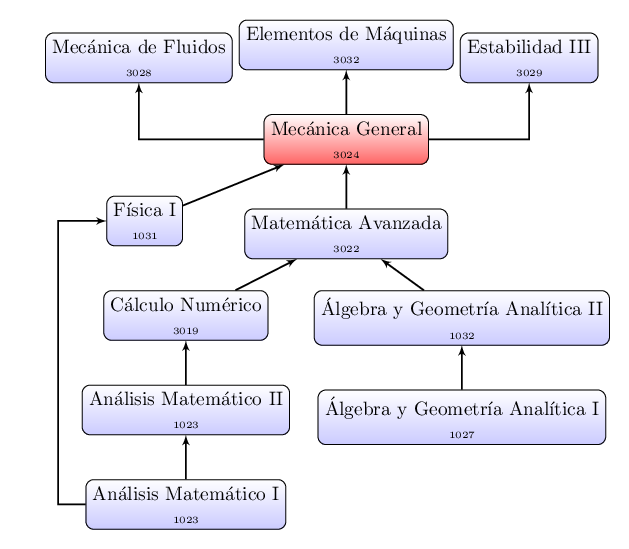
\includegraphics[width=3in]{figuras/correlativas.png}
\caption{Preceded by subjects of algebra, analysis, and physics, General Mechanics is the first in which such knowledge is applied to mechanical engineering.}
\label{fig:correlativas}
\end{figure}

The subject trains students in the ability to model the physics of simple mechanical systems. Modeling is understood as a series of procedures with which a simplified scheme of physics is constructed based on a semi-quantitative evaluation of the forces and fields that act on the system as well as the constraints that limit its degrees of freedom. With such information, some of these are prioritized and others are discarded to arrive at the aforementioned scheme. Having such a model allows:
\begin{itemize}
    \item to choose generalized coordinates to describe the relevant degrees of freedom,
    \item to write mathematical relationships between them that account for constraints,
    \item to describe generalized forces that are not the effect of fields (gravitational, electromagnetic, etc.),
    \item and to describe the potential and kinetic energy of the system as a whole.
\end{itemize}


After performing the above, the Euler-Lagrange formalism is demonstrated and put into practice in the course to obtain a set of differential equations that describe the dynamics of the system and/or the mechanical stresses that each of its components must withstand at each instant of time.

From what has been exposed in the preceding paragraphs, it is evident that the subject matter of the course object of this work is circumscribed to the conventional one of rational mechanics courses as detailed in its canonical reference literature \cite{landau}. It is not in the subject matter but in its didactic methodology where innovation was made.

\subsection{The blackboard, the only didactic tool}

Traditionally, the systems worked on in rational mechanics courses are relatively simple to limit the time and/or difficulty of mathematical analysis and/or algebra calculations required by the steps commented in the previous paragraph. But this extreme simplification leads to a noticeable jump in the complexity required to model mechanical devices, fluid dynamics, or rigid structures, the respective subjects of the courses subsequent to General Mechanics (see Figure \ref{fig:correlativas}).

The limitation to complexity is imposed by what the teacher can calculate on the blackboard during a class. As they are erased successively, they not only prevent the student from using a reference of something that is no longer in sight, but also impose on them to devote a good part of their attention to not making mistakes when transcribing what is written there into their notebook. This paper support, in turn, limits the length and complexity of the problems that can be proposed to students to exercise what they have learned. What summarizes the preceding paragraph is nothing more than the procedure in the teaching of science or engineering courses at the university level that has been almost unchanged since the 19th century to the present day.


\subsection{Computer-based didactic tools}

The steps before and after obtaining a system of differential equations that describe the dynamics and stresses for a complex mechanical model can be performed with computer-based tools, but they are different for each case. To solve and analyze the result of the equations, the tools learned in the Numerical Calculus subject, previously taken before General Mechanics, and ubiquitous graphing tools to visualize the temporal evolution of different magnitudes are applied. Although it is true that numerical calculus is occasionally used in exercises \cite{mirasso-raichman, caligaris-rodriguez}, it is rarely used by the teacher during class. This is a missed opportunity to better exemplify and deepen the analysis of the behavior of the modeled systems.

But if the application of numerical calculus during classes is rare, the use of computer algebra systems (CAS) is even rarer. These systems allow automating all the mathematical procedures required for modeling: from defining degrees of freedom, coordinate systems, fields, and external forces to the model to building the system of differential equations for the dynamics. Using them to solve linear algebra and mathematical analysis calculations allows to remove the emphasis on these and focus the attention of the teacher and students on the subject matter of the course.

However, the daily reality of our classrooms is that these calculations continue to be done manually on the blackboard or on paper during classes, ignoring the use of computers. Insisting on this procedure at the university level would be analogous to depriving students of the use of pocket calculators to perform arithmetic procedures learned at the primary level. It is an anachronism in the third decade of the 21st century.

\subsection{Code recycling}

The above can be misinterpreted as a mere call to use computers as an analog of the pocket calculator, replacing the results of the calculations required to solve exercises on paper. This would be an underutilization of such a resource in the class, repeating the pattern followed by most computer users who ignore a fundamental aspect of computing in their daily use.

The digital computer was invented during World War II to perform numerical calculations that were manually defined in each execution, operating as a faster calculator with the ability to automate some of the numerical manipulation processes. But since the middle of the last century, it has acquired the ability to operate under a series of instructions stored in its memory on how to process both numerical and other information. Such instructions are called programs, and they are written in a code that respects the syntax of a certain language.

Modern high-level languages allow writing a single code incorporating all the procedures required for the resolution and analysis of a rational mechanics problem. This includes from the assumptions made to simplify the physics of the problem to the analysis with graphs of its dynamics and mechanical stresses, passing through all the intermediate algebraic and numerical calculations.

Starting from the objective that students exploit this tool, the course had as its methodology to avoid paper work and instead develop the ability to write in a single code the set of operations required to solve exercises. In class, the teacher explained synchronously examples of codes that perform all the procedures required to model a mechanical system. In each class, a guide to solvable exercises is provided by making small modifications to the code.














% En el plan de la carrera de grado en Ingeniería Mecánica del Departamento de Ingeniería e Investigaciones Tecnológicas (DIIT) de la UNLaM esta asignatura es el nexo entre las primeras propias de la especialidad con las básicas en las que se imparten herramientas de álgebra, análisis matemático, cálculo numérico, y mecánica Newtoniana. El esquema de correlatividades inmediatas a la asignatura Mecánica General, que muestra la figura \ref{fig:correlativas}, deja en claro que esta debe tener entre sus objetivos el mostrar al alumno cómo dichas herramientas tienen aplicación en su tema de interés.

% \begin{figure}[!ht]
% \centering
% 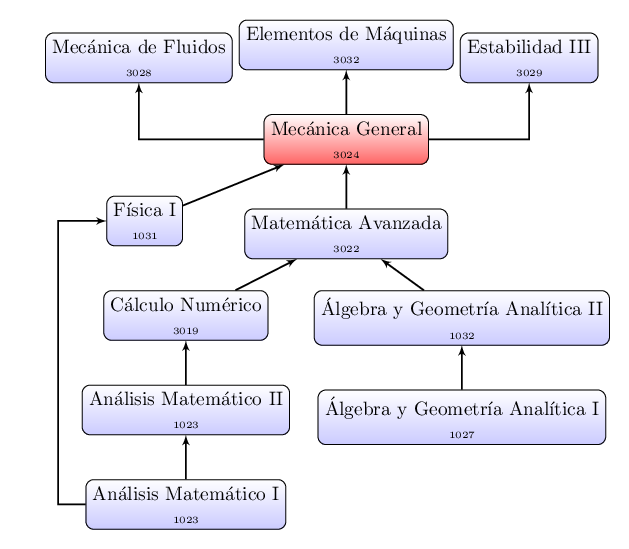
\includegraphics[width=3in]{figuras/correlativas.png}
% \caption{Precedida de asignaturas de álgebra, análisis y física, Mecánica General es la primera en que se aplican tales conocimientos a la ingeniería mecánica.}
% \label{fig:correlativas}
% \end{figure}

% La asignatura entrena a los alumnos en la habilidad de modelizar la física de sistemas mecánicos simples. Se entiende por modelizar el realizar una serie de procedimientos con los que se construye un esquema simplificado de la física partiendo de una evaluación semi-cuantitativa de las fuerzas y campos que actúan sobre el sistema así como de las ligaduras que limitan sus grados de libertad. Con tal información se priorizan algunas de estas y se descartan otras para arribar al esquema mencionado. Disponer de tal modelo permite:
% \begin{itemize}
%     \item elegir coordenadas generalizadas para describir los grados de libertad relevantes,
%     \item escribir relaciones matemáticas entre estas que den cuenta de ligaduras,
%     \item describir las fuerzas generalizadas que no sean efecto de campos (gravitatorio, electromagnéticos, etc.),
%     \item y describir la energía potencial y cinética del sistema en su conjunto.
% \end{itemize}

% Tras realizar lo anterior se demuestra y se pone en práctica en el curso el formalismo de Euler-Lagrange para obtener un conjunto de ecuaciones diferenciales que describen la dinámica del sistema y/o los esfuerzos mecánicos que cada uno de sus componentes debe soportar en cada instante de tiempo.

% De lo expuesto en los párrafos precedentes se evidencia que la temática del curso objeto de este trabajo está circunscrita a la convencional de los cursos de mecánica racional como se detalla en su literatura canónica de referencia \cite{landau}. No es en la temática sino en su metodología didáctica donde se hizo una innovación.

% \subsection{El pizarrón, única herramienta didáctica}

% Tradicionalmente los sistemas que se trabajan en los cursos de mecánica racional son relativamente simples para acotar el tiempo y/o dificultad de los cálculos de análisis matemático y/o de álgebra que requieren los pasos comentados en el párrafo anterior. Pero esta simplificación extrema lleva a un notorio salto en la complejidad de la que requiere modelar de dispositivos mecánicos, la dinámica de fluidos o a estructuras rígidas, las respectivas temáticas de las asignaturas subsiguientes a Mecánica General (ver figura \ref{fig:correlativas}).

% La limitación a la complejidad la impone lo que el docente puede, en la duración de una clase, calcular en el pizarrón. Estos al irse borrando sucesivamente no sólo impide al alumno servirse de referencia de algo que ya no está a la vista sino que además le impone dedicar buena parte de su atención a no cometer errores al transcribir lo allí escrito en su cuaderno. Este soporte en papel a su vez limita la extensión y complejidad de los problemas que pueden proponerse al alumnado para ejercitar lo aprendido. 
% Lo  que sintetiza el párrafo precedente no es otra cosa que el proceder en el dictado de clases de ciencias o ingeniería a nivel universitario que se reproduce casi en forma inalterada desde el siglo XIX hasta nuestros días.

% \subsection{Herramientas didácticas informáticas}

% Los pasos previos y posteriores al obtener un sistema de ecuaciones diferenciales que describen la dinámica y esfuerzos para un modelo mecánico complejo pueden realizarse con herramientas informáticas, pero que son distintas para cada caso.
% Para resolver y analizar el resultado de las ecuaciones se aplican las herramientas aprendidas en la asignatura Cálculo Numérico, cursada previamente a Mecánica General, y las ubicuas de graficación para visualizar la evolución temporal de distintas magnitudes. Si bien es cierto que el cálculo numérico se aprovecha ocasionalmente en la ejercitación \cite{mirasso-raichman, caligaris-rodriguez}, este rara vez es utilizado por el docente durante la clase. Se pierde así una oportunidad de ejemplificar mejor y profundizar el análisis del comportamiento de los sistemas modelados.

% Pero si es rara la aplicación del cálculo numérico durante las clases lo es aún más el uso de sistemas de álgebra computacional (Computer Algebra Systems o CAS, en inglés), que permiten automatizar todos los procedimientos matemáticos que requiere la modelización: desde definir grados de libertad, sistema de coordenadas, campos y fuerzas externas al modelo hasta construir el sistema de ecuaciones diferenciales para la dinámica. El utilizarlos para resolver cálculos de álgebra lineal y análisis matemático permite quitar el énfasis sobre estos y centrar la atención del docente y alumnos en la temática propia de la asignatura.

% Pero la realidad cotidiana de nuestras aulas es que durante las clases dichos cálculos se continúan realizando manualmente en el pizarrón o en papel obviando el uso de la informática. Empeñarse en ese proceder en el nivel universitario sería análogo al de privar al alumnado del uso de calculadoras de bolsillo para realizar procedimientos aritméticos aprendidos en el nivel primario. Todo un anacronismo en la tercera década del siglo XXI.

% \subsection{Reciclado del código}

% Lo precedente puede interpretarse erróneamente como un mero llamado a utilizar la informática como un análogo de la calculadora de bolsillo, supliendo resultados de los cálculos que demanda la resolución de ejercicios en papel. Eso sería una infrautilización de tal recurso en la clase, repitiendo el patrón que sigue la mayor parte de los usuarios de computadoras que obvian en su uso cotidiano un aspecto fundamental de la informática.

% La computadora digital se inventó en la Segunda Guerra Mundial con el fin de realizar cálculos numéricos que se definían manualmente en cada ejecución operando como una calculadora más rápida y con capacidad de automatizar algunos de los procesos de manipulación numérica.  Pero desde la mitad del siglo pasado adquirió la capacidad de operar bajo una serie de instrucciones almacenadas en su memoria sobre cómo procesar información tanto numérica como de otra índole. Tales instrucciones reciben el nombre de programa, y se escriben en un código que respeta la sintaxis de un determinado lenguaje.

% Los lenguajes modernos de alto nivel permiten escribir un único código incorporando  todos los procedimientos que requiere la resolución y el análisis de un problema de mecánica racional. Esto abarca desde las aproximaciones asumidas para simplificar la física del mismo hasta el análisis con gráficas de su dinámica y esfuerzos mecánicos pasando por todos los cálculos algebraicos y numéricos intermedios.

% Partiendo del objetivo de que los alumnos exploten esta herramienta el curso tuvo por metodología el obviar el trabajo en papel y en su lugar desarrollar la habilidad de escribir en un único código el conjunto de operaciones que requiere la resolución de ejercicios. En clase el docente explicó en forma sincrónica ejemplos de códigos que realizan todos los procedimientos requeridos para modelar un sistema mecánico. En cada clase se provee una guía de ejercicios resolubles haciendo pequeñas modificaciones al código provisto por el docente en esa fecha. Sucesivos ejercicios de complejidad creciente requieren pequeñas modificaciones respecto al código con que se resolvió el anterior. Esta reutilización del código permite un mejor aprovechamiento del tiempo y esfuerzo del alumno que en resoluciones en papel donde debe repetir procedimientos ya realizados en anteriores oportunidades. Clase a clase el alumnado construye una biblioteca de códigos con capacidades crecientes de análisis \cite{Barba2019}.

% Hay que aclarar que no se forma al alumno en programación para que cree aplicaciones o algoritmos, lo que se denomina programming en inglés. Lo que se busca es que puedan codificar  (por coding en inglés) las instrucciones para que la computadora realice tareas específicas, en particular cálculos para la ingeniería mecánica.

% Algunos alumnos archivan sus resoluciones de ejercicios resueltas en papel como referencia en caso de que se presente una problemática similar más adelante en el cursado de la carrera o en la vida profesional. En los hechos esto rara vez sucede y si recurren en el futuro a algún material relacionado a la asignatura es a su bibliografía, que por lo expuesto anteriormente carece de ejemplos adaptables a modelos más complejos que los comúnmente tratados en la asignatura. Por contrapartida un código es fácilmente aplicable al análisis de una problemática profesional análoga a las vistas en el curso. Al figurar en forma explícita las instrucciones para realizar cada paso del procedimiento es sencillo de revisar, expandir y modificar.

\section{Tools used on this curse}

Here is the translation of the technical text you provided:

\subsection{Python, Sympy, Numpy, Scipy and Matplotlib}

The Python programming language is by default devoid of scientific and engineering calculation capabilities. This is a design decision to make such functionalities be added by specialized libraries. The effect of this decision is that the development of these libraries is carried out by users who apply them in various fields of scientific-technological development rather than by computer professionals.

The functions of symbolic calculation are provided by the Sympy library. Its Mechanics module is particularly useful for generating equations for the dynamics of rigid body systems with multiple degrees of freedom and in various reference systems \cite{simpy}.

Differential equation systems are solved by numerical methods supported by functions for the manipulation of algebraic elements of the Numpy library \cite{numpy} and the numerical optimization and integration algorithms of Scipy \cite{SciPy}.

Engineering analysis of numerical results is usually interpreted with graphical representations. This capability is provided by the functions of the Matplotilb library \cite{matplotlib}.

\subsection{Jupyter Notebooks}

The environment used in the course to run code is the web-based application of the Jupyter Project called JupyterLab, whose document format is the Jupyter notebook \cite{Kluyver2016jupyter}. This alternates independent sections called cells. Input cells are code (in various languages, Python is just one of the possibilities) or annotations, as shown in Figure \ref{fig:jupyter}. This latter variant of cells is written in the Markdown markup language \cite{markdown} that allows you to embed: text and/or mathematical expressions in \LaTeX format interspersed, and multimedia content: web links, images, video and/or sound players.


Here is the translation of the technical text you provided:

\subsection{Python, Sympy, Numpy, Scipy and Matplotlib}

The Python programming language is by default devoid of scientific and engineering calculation capabilities. This is a design decision to make such functionalities be added by specialized libraries. The effect of this decision is that the development of these libraries is carried out by users who apply them in various fields of scientific-technological development rather than by computer professionals.

The functions of symbolic calculation are provided by the Sympy library. Its Mechanics module is particularly useful for generating equations for the dynamics of rigid body systems with multiple degrees of freedom and in various reference systems \cite{simpy}.

Differential equation systems are solved by numerical methods supported by functions for the manipulation of algebraic elements of the Numpy library \cite{numpy} and the numerical optimization and integration algorithms of Scipy \cite{SciPy}.

Engineering analysis of numerical results is usually interpreted with graphical representations. This capability is provided by the functions of the Matplotilb library \cite{matplotlib}.

\subsection{Jupyter Notebooks}

The environment used in the course to run code is the web-based application of the Jupyter Project called JupyterLab, whose document format is the Jupyter notebook \cite{Kluyver2016jupyter}. This alternates independent sections called cells. Input cells are code (in various languages, Python is just one of the possibilities) or annotations, as shown in Figure \ref{fig:jupyter}. This latter variant of cells is written in the Markdown markup language \cite{markdown} that allows you to embed: text and/or mathematical expressions in \LaTeX format interspersed, and multimedia content: web links, images, video or sound players..

\subsection{Running Jupyter Online}

Students are not required to install any software on their computer to take the course. They only need to use a standard web browser to use one of the services that run Jupyter notebooks online. This can be an installation of JupyterHub from the Jupyter Project on university-owned servers or commercial clouds, or alternatively one of the services that offer even free alternatives such as CoCalc, IBM Watson or Google Colaboratory. Of these, the latter has been used in the latest editions of the course after Microsoft closed its free Azure Notebooks service.

Here is the translation of the technical text you provided:

\subsection{Python, Sympy, Numpy, Scipy and Matplotlib}

The Python programming language is by default devoid of scientific and engineering calculation capabilities. This is a design decision to make such functionalities be added by specialized libraries. The effect of this decision is that the development of these libraries is carried out by users who apply them in various fields of scientific-technological development rather than by computer professionals.

The functions of symbolic calculation are provided by the Sympy library. Its Mechanics module is particularly useful for generating equations for the dynamics of rigid body systems with multiple degrees of freedom and in various reference systems \cite{simpy}.

Differential equation systems are solved by numerical methods supported by functions for the manipulation of algebraic elements of the Numpy library \cite{numpy} and the numerical optimization and integration algorithms of Scipy \cite{SciPy}.

Engineering analysis of numerical results is usually interpreted with graphical representations. This capability is provided by the functions of the Matplotilb library \cite{matplotlib}.

\subsection{Jupyter Notebooks}

The environment used in the course to run code is the web-based application of the Jupyter Project called JupyterLab, whose document format is the Jupyter notebook \cite{Kluyver2016jupyter}. This alternates independent sections called cells. Input cells are code (in various languages, Python is just one of the possibilities) or annotations, as shown in Figure \ref{fig:jupyter}. This latter variant of cells is written in the Markdown markup language \cite{markdown} that allows you to embed: text and/or mathematical expressions in \LaTeX format interspersed, and multimedia content: web links, images, video or sound players..

\subsection{Running Jupyter Online}

Students are not required to install any software on their computer to take the course. They only need to use a standard web browser to use one of the services that run Jupyter notebooks online. This can be an installation of JupyterHub from the Jupyter Project on university-owned servers or commercial clouds, or alternatively one of the services that offer even free alternatives such as CoCalc, IBM Watson or Google Colaboratory. Of these, the latter has been used in the latest editions of the course after Microsoft closed its free Azure Notebooks service.

The Google Colaboratory service, colloquially only Colab, presents as a convenience the ability to run notebooks hosted in a Git repository managed by the online service GitHub. A modification in the URL is enough to point a notebook to a web browser to run it in Colab \cite{colab}. Working with Jupyter notebooks in this service can be done concurrently by several students and/or teachers. Comments can also be included, whose update is reported by email, which is useful for correcting exercises since the location of errors in the code can be indicated, as shown in Figure \ref{fig:colab}.

\subsection{Git Repository}

The aforementioned repository on GitHub is organized into separate folders for each class of the course, as shown in Figure \ref{fig:github}. Each of these hosts the corresponding theoretical material and exercises in the format of Jupyter notebooks, as well as exercise guides and occasional notes in the portable document format known by its acronym in English PDF. This arrangement facilitates both the teacher and the students an overview of the material of each topic as well as verifying any updates to it. In this way, the course material is publicly accessible, making it available for use by interested parties \cite{repositorio-victor} as long as they cite its origin and do not use it commercially as indicated by its Creative Commons CC-BY-NC-SA license under which it is published \cite{creative}.

Here is the translation of the technical text you provided:

\begin{figure}[!ht]
\centering
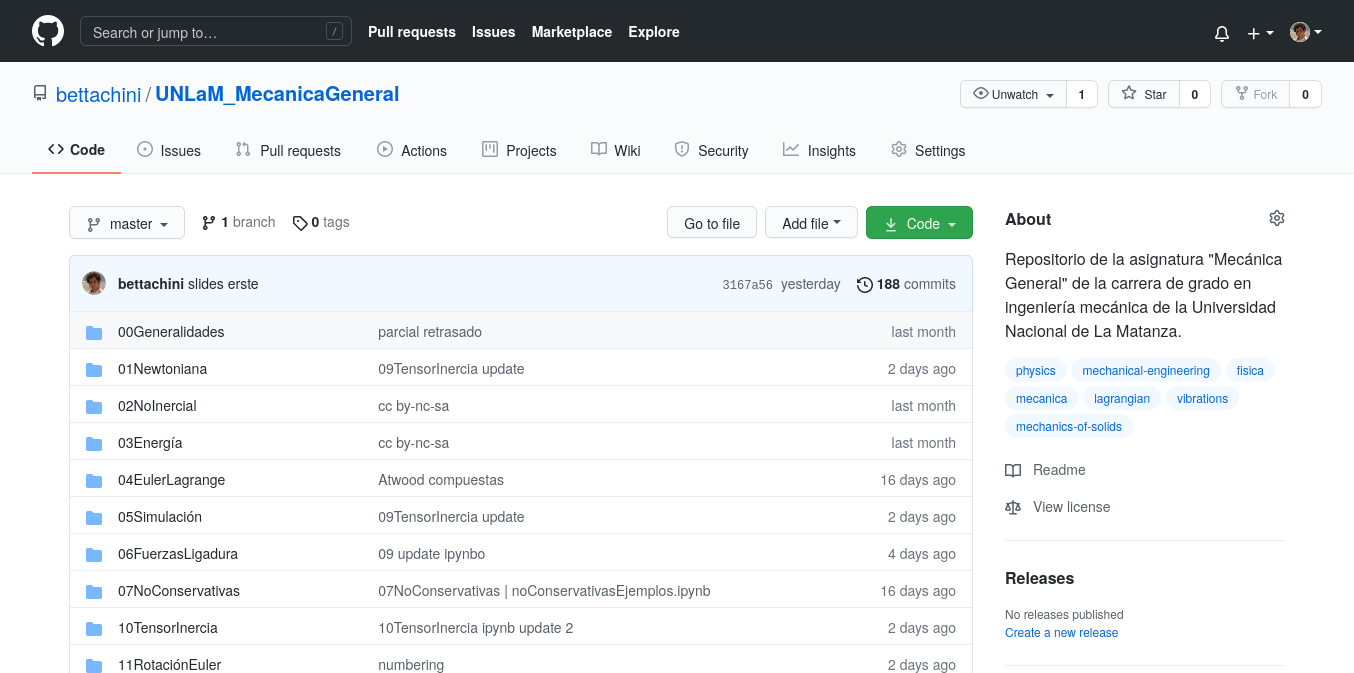
\includegraphics[width=3.5in]{figuras/repositorioGithub.png}
\caption{The students find the material organized in separate directories per class.}
\label{fig:github}
\end{figure}

\subsection{Learning Management System}

At UNLaM, the Microsoft Teams business communications platform is used to replace classroom interaction with students with videoconferencing. After each class, the videos are saved to Microsoft OneDrive online storage. Links to these and to the class materials hosted in the Git repository are compartmentalized into what the system calls channels, respecting the same numbering and naming as in the Git repository. Figure \ref{fig:teams} shows the contents that head the ones displayed for the tenth class.

Each channel includes links to:
\begin{itemize}
    \item practical exercise guide
    \item any occasional notes in PDF
    \item both ways to view Jupyter notebooks, interactive in Colab or static in nbviewer
    \item invitation to the videoconference or its video once it is over
\end{itemize}

Microsoft Teams also provides the rudiments of a Learning Management System (LMS) by allowing tasks to be assigned to students with acceptance deadlines by the system. Students can upload a link to their Colab notebook or the same in .ipynb format if modification is not allowed after a certain date for evaluation purposes.

\begin{figure}[!ht]
\centering
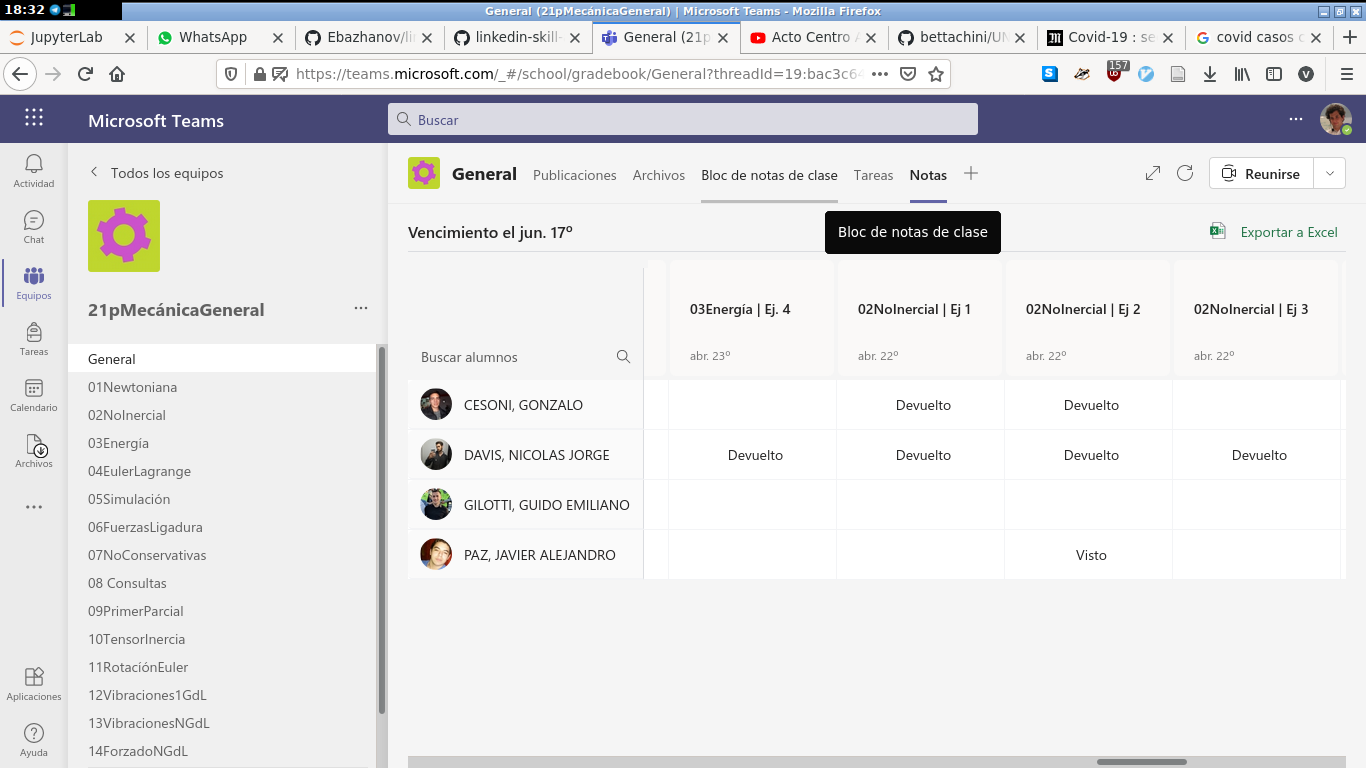
\includegraphics[width=3.5in]{figuras/notasTeams.png}
\caption{Separate channels per class present links to their material.}
\label{fig:teams}
\end{figure}




















% \subsection{Python, Sympy, Numpy, Scipy y Matplotlib}

% El lenguaje de programación Python está por defecto desprovisto de capacidades de cálculo científico e ingenieril.  Esta es una decisión de diseño para hacer que tales funcionalidades deban ser agregadas por bibliotecas especializadas. El efecto de esta decisión es que el desarrollo de las mismas corre por cuenta de usuarios que las aplican en diversos ámbitos del desarrollo científico-tecnológico antes que por profesionales de las informática.

% Las funciones del cálculo simbólico las provee la biblioteca Sympy. Se aprovecha en particular su módulo Mechanics que facilita la generación de ecuaciones para la dinámica de sistemas de cuerpos rígidos con múltiples grados de libertad y en variados sistemas de referencia \cite{simpy}.

% Los sistemas de ecuaciones diferenciales se resuelven por métodos numéricos apoyados en las funciones para la manipulación de elementos algebraicos de la biblioteca Numpy \cite{numpy} y de los algoritmos de optimización e integración numérica de Scipy \cite{SciPy}.

% El análisis en ingeniería de resultados numéricos son usualmente interpretados con representaciones gráficas. Esta capacidad la proveen las funciones de la biblioteca Matplotilb \cite{matplotlib}.

% \subsection{Cuadernos de Jupyter}

% El entorno usado en el curso para ejecutar código es la aplicación basada en la web del Proyecto Jupyter llamada JupyterLab cuyo  formato de documento es el cuaderno (notebook) Jupyter \cite{Kluyver2016jupyter}. Este alterna secciones independientes denominadas celdas. Las de entrada son de código (en variados lenguajes, Python es solo uno de los posibles) o de  anotaciones, como muestra la figura \ref{fig:jupyter}. Esta última variante de celdas se escriben en el lenguaje de  marcado Markdown \cite{markdown} que permite incrustar: texto y/o expresiones matemáticas en formato \LaTeX intercaladas, y contenido multimedia: enlaces web, imágenes, reproductores de video o sonido.

% \begin{figure}[!ht]
% \centering
% 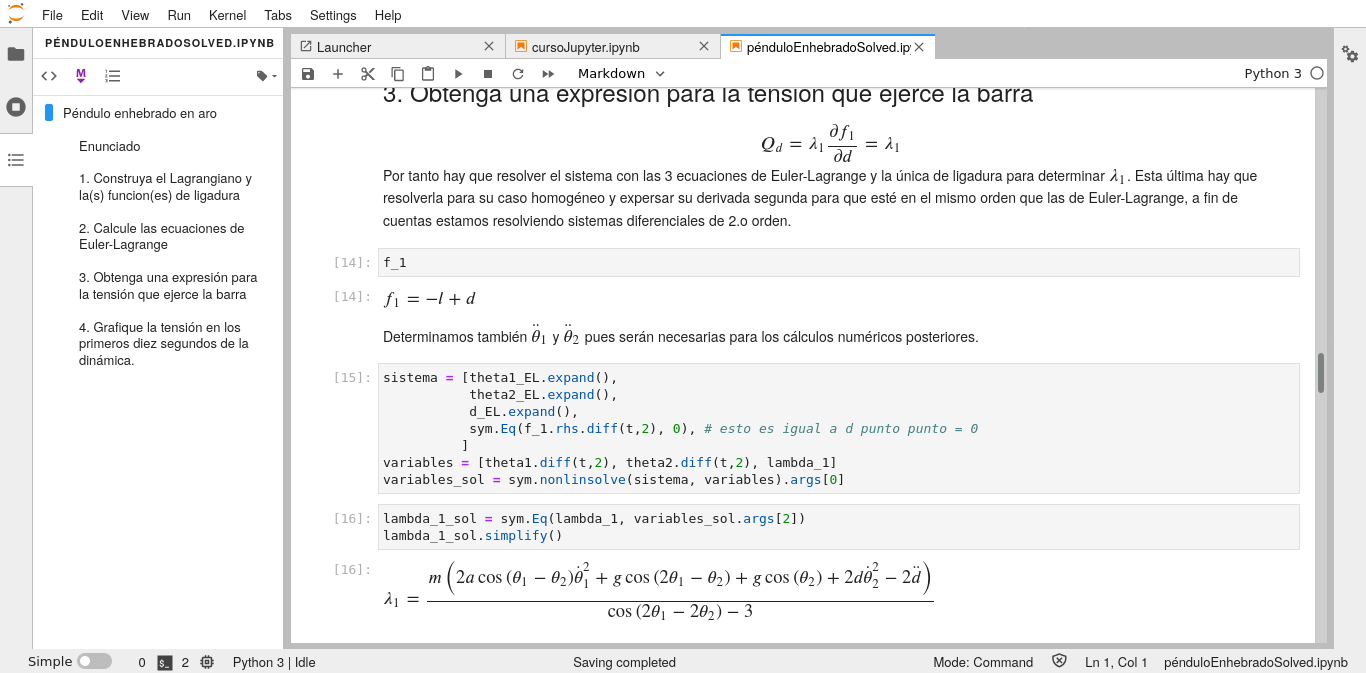
\includegraphics[width=3.5in]{figuras/screenshot_JupyterLab.png}
% \caption{Un cuaderno de Jupyter es un conjunto de celdas. Estas son en formato Markdown o de código ejecutable. Las primeras pueden contener texto,  expresiones  matemáticas o contenido multimedia. Las segundas líneas de código en variados lenguajes de programación. Intercalando títulos en las celdas Markdown se genera el índice (a la izquierda) que facilita la ubicación dentro del documento.}
% \label{fig:jupyter}
% \end{figure}

% La utilización de sintaxis \LaTeX para la simbología matemática provee una notación clara estandarizada bajo los lineamientos de la American Mathematical Society \cite{ams}.
% El resultado de la ejecución de una celda de código muestra al usuario el resultado que el mismo instruye a la computadora imprimir. En el curso estas últimas incluyen tanto los comandos para realizar cálculos así como la resolución de un sistema de ecuaciones no lineales que se imprime en la última celda del cuaderno mostrado en la figura 2.  

% \subsection{Ejecución de Jupyter en línea}

% No se impone a los estudiantes el instalar ningún software para cursar la materia en su dispositivo informático. Solo requieren utilizar un navegador web estándar para utilizar alguno de los servicios que ejecutan cuadernos de Jupyter en línea. Este puede tratarse de una instalación de JupyterHub del Proyecto Jupyter en servidores propios de la universidad o en nubes comerciales, o en su defecto de alguno de los servicios que ofrecen alternativas incluso gratuitas como, entre otras, CoCalc, IBM Watson o Google Colaboratory. De estas se ha utilizado esta última en las últimas ediciones del curso tras cerrar Microsoft su servicio gratuito Azure Notebooks.

% El servicio Google Colaboratory, coloquialmente sólo Colab,  presenta como conveniencia el poder ejecutar cuadernos alojados en un repositorio Git gerenciado por el servicio en línea GitHub. Basta una modificación en el URL de un cuaderno para que este apunte a un navegador web a ejecutarle en Colab \cite{colab}. El trabajo con cuadernos Jupyter en este servicio puede realizarse en forma concurrente por parte de varios alumnos y/o docentes. También pueden incluirse comentarios cuya actualización es reportada por correo electrónico lo que es útil para la corrección de los ejercicios pues pueden indicarse la ubicación de errores en el código como muestra la figura \ref{fig:colab}.

% \begin{figure}[!ht]
% \centering
% 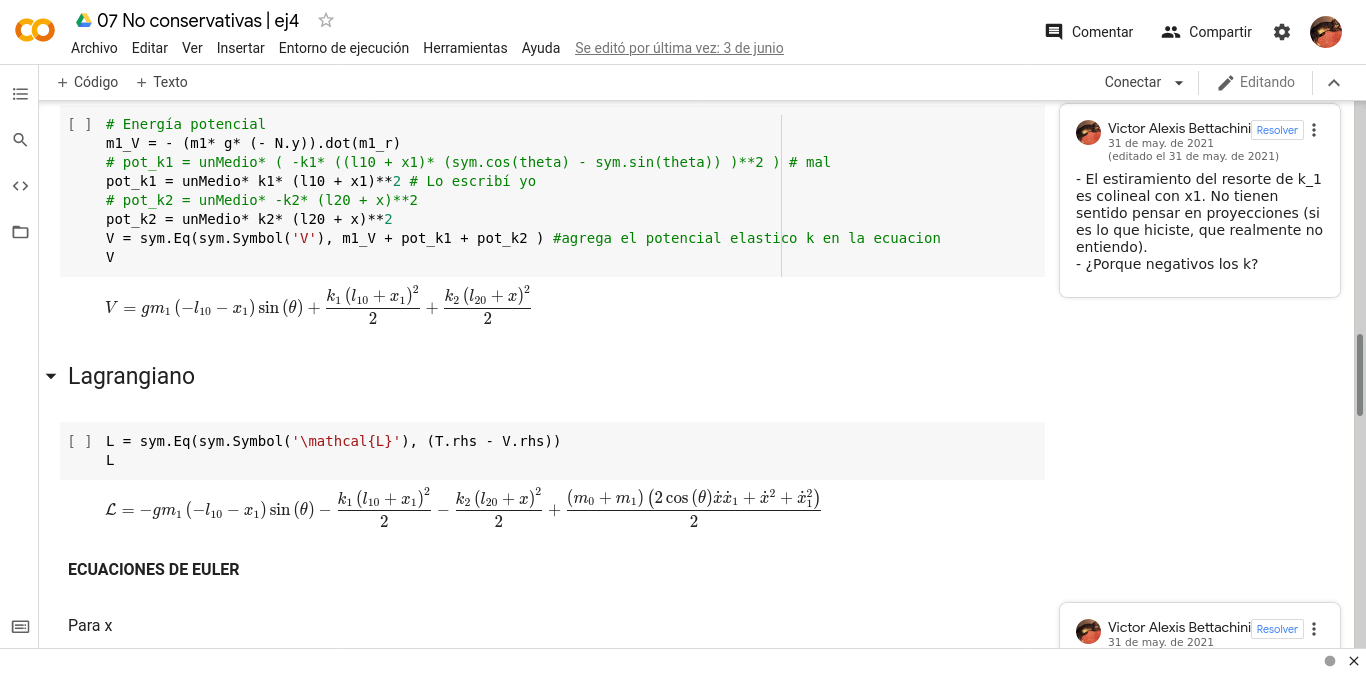
\includegraphics[width=3.5in]{figuras/comentariosColab.png}
% \caption{El sitio web Google Colaboratoy permite editar y ejecutar cuadernos Jupyter en forma concurrente entre alumnos y docentes además de incluir comentarios. Esta última característica es útil para las correcciones.}
% \label{fig:colab}
% \end{figure}

% \subsection{Repositorio Git}

% El mencionado repositorio en GitHub está organizado en sendas carpetas por clase del curso, como muestra la figura \ref{fig:github}. Cada una de estas aloja el correspondiente material teórico y ejercicios en el formato de cuadernos Jupyter además de  guías de ejercicios y algún apunte ocasional en el formato de documento portátil conocido por su sigla en inglés PDF. Este ordenamiento facilita tanto al docente como a los alumnos una vista de conjunto del material de cada temática así como el verificar las eventuales actualizaciones del mismo. De esta forma el material del curso es de acceso público haciéndolo disponible para ser utilizado a interesados \cite{repositorio-victor} mientras cumplan con citar su origen y no darle uso comercial como indica su licencia Creative Commons CC-BY-NC-SA bajo el que está publicado \cite{creative}.

% \begin{figure}[!ht]
% \centering
% 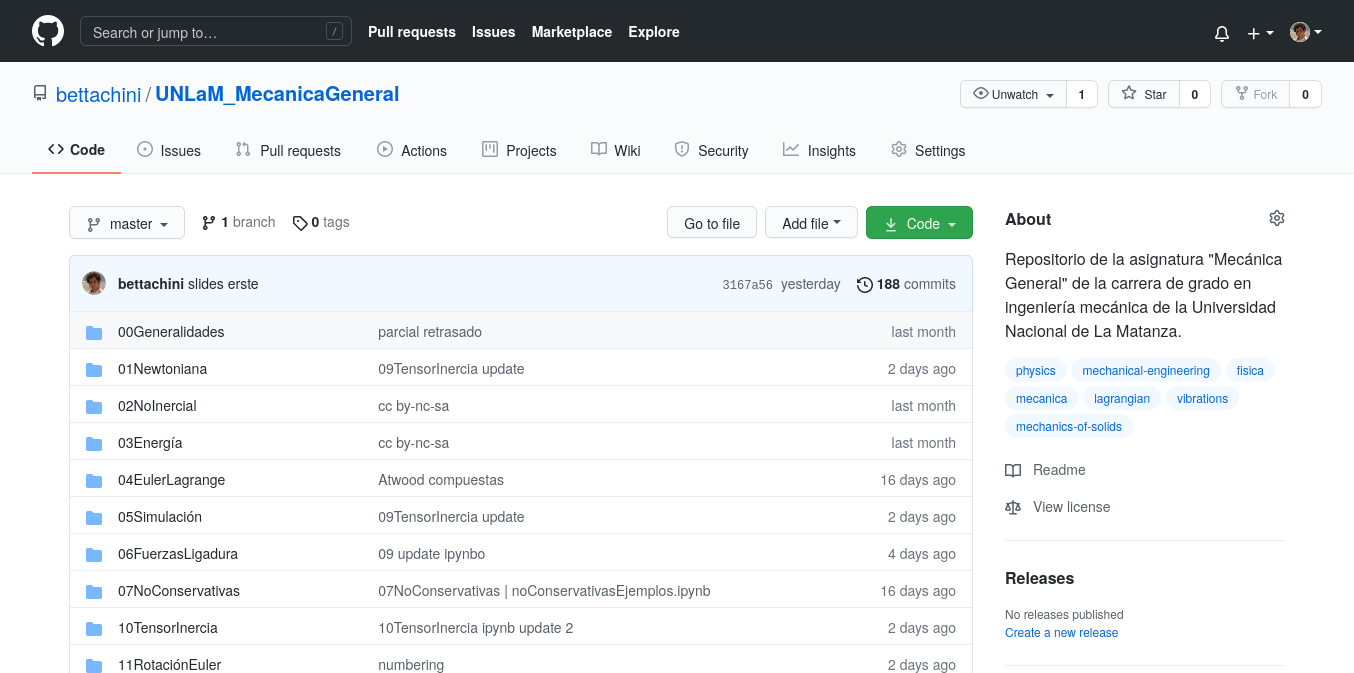
\includegraphics[width=3.5in]{figuras/repositorioGithub.png}
% \caption{Los alumnos encuentran el material ordenado en sendos directorios por clase.}
% \label{fig:github}
% \end{figure}

% \subsection{Sistema de gestión de aprendizaje}

% En la UNLaM se utiliza la plataforma de comunicaciones de negocios Microsoft Teams para suplir la interacción en el aula con los alumnos con videoconferencias. Luego de terminada cada clase el video de las mismas se guarda en el almacenamiento en línea Microsoft OneDrive. Enlaces a estos y a los materiales de la clase alojados en el repositorio Git se  compartimentan en lo que el sistema llama canales respetando la misma numeración y denominación que en el repositorio Git. La figura \ref{fig:teams} muestra los contenidos que encabezan los desplegados para la décima clase.

% En cada canal se incluyen enlaces a:
% \begin{itemize}
%     \item guía de ejercicios prácticos
%     \item algún eventual apunte en PDF
%     \item ambas vías para ver los cuadernos Jupyter, la interactiva en Colab o estática en nbviewer
%     \item invitación a la videoconferencia o a su video una vez esta terminó
% \end{itemize}

% Microsoft Teams provee también los rudimentos de un sistema de gestión de aprendizaje (LMS por sus siglas en inglés) al permitir asignar tareas a alumnos con fechas límites de aceptación por parte del sistema. Los alumnos pueden cargar al sistema un enlace a su cuaderno en Colab o el mismo en formato .ipynb en el caso de que no se permita modificación del mismo con posterioridad a una fecha por cuestiones de evaluación.

% \begin{figure}[!ht]
% \centering
% 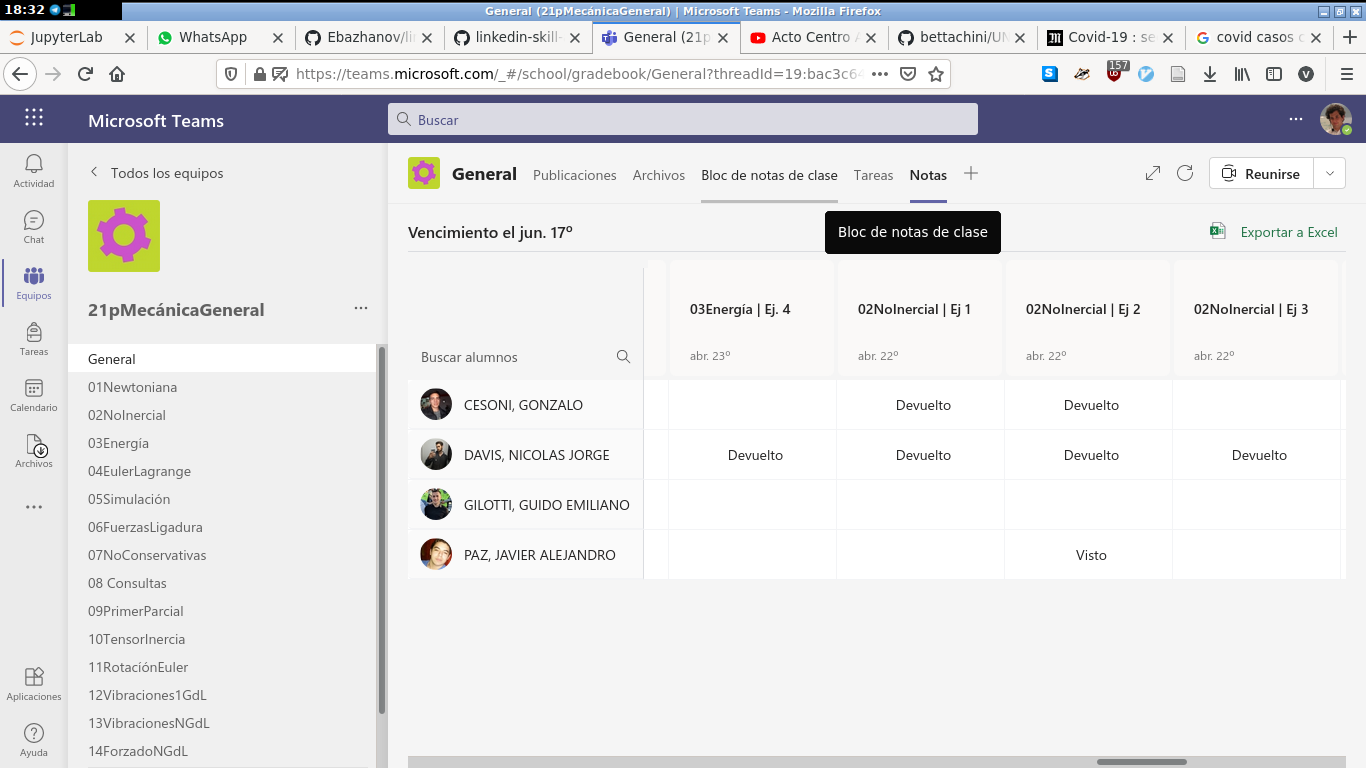
\includegraphics[width=3.5in]{figuras/notasTeams.png}
% \caption{Sendos canales por clase presentan los enlaces a su material.}
% \label{fig:teams}
% \end{figure}

\section{Cruse chronology}

Out of the 16 weekly meetings throughout a semester, 13 present new topics.
By the end of the second week generalised coordinates were used to calculate the mechanical energy of various systems with ad-hoc Sympy-based functions provided by the teaching staff.
From third to fifth week the Euler-Lagrange approach is implemented into code to simulate the dynamics of multiple point mass systems.
By the eighth week, constrained forces and non-conservative ones are calculated.
Starting at the ninth week the course focus on extended bodies modelled as rigid bodies employing inertia tensors and Euler equations for rotation.
The final weeks are devoted to vibrations including forced harmonic oscillations and modal analysis at systems with multiple degrees of freedom.
Further details beyond this brief description of the weekly topics can be obtained from the full schedule available at the course repository \cite{repositorio-victor}.
The progression of the course is illustrated by the following selection of some of these topics.


\textbf{Week 1: vector kinematics}
After a brief introduction to the flipped classroom methodology and description of the coding tools to use, a hand-on practice on the use of Google Colab begins.
As a first exposure to Sympy calculus capabilities, students are presented with a review of vector kinematics with code for time-differention of position vector in some reference frames and coordinate systems as shown in figure \ref{fig:week1_differentiation}.

\begin{figure}[!ht]
    \centering
    \includegraphics[width=0.95\linewidth]{figuras/week1_differentiation.png}
    \caption{The first lesson in Jupyter notebooks: a review of kinematics where Sympy calculus functions are used.}
    \label{fig:week1_differentiation}
\end{figure}

Then in a second lesson notebook the construction of a function to calculate the kinetic energy for a compound pendulum is explained step-wise. 
Students are encouraged to review the \LaTeX\ notation used in that notebook.


\textbf{Week 3: Euler-Lagrange formalism}
This is the main tool of analytical mechanics that students will instrumentalise to generate diffential equations to describe, at this stage of the course, the dynamics of multiple point mass systems.
After a step-wise construction, akin that followed with functions for energies, a function to generate these equations is provided to the student in an example problem as illustrated by figure \ref{fig:week4_eulerLagrangeFunction}.
This code will be re-used by the student from now on through the course to address problems at every exercises set.

\begin{figure}[ht]
    \centering
    \includegraphics[width=\linewidth]{figuras/week4_eulerLagrangeFunction.png}
    \caption{The Euler-Lagrange formalism is the center piece of the analytical tools used in the course. After a step by step construction, a fully assembled function would allow to apply it in code used thereafter.}
    \label{fig:week4_eulerLagrangeFunction}
\end{figure}


So far, code has been used to perform the same steps that are solved on a blackboard or paper in a conventional rational mechanics course to arrive at differential equations that are only solved for trivial cases.
In contrast, using Sympy quickly solves complex systems for acceleration a function of generalized coordinates and velocities as shown in Figure \ref{fig:clase4ac}.
Performing such a task manually would require a non-negligible amount of time and effort even for this system with only two degrees of freedom.

\begin{figure}[!ht]
\centering
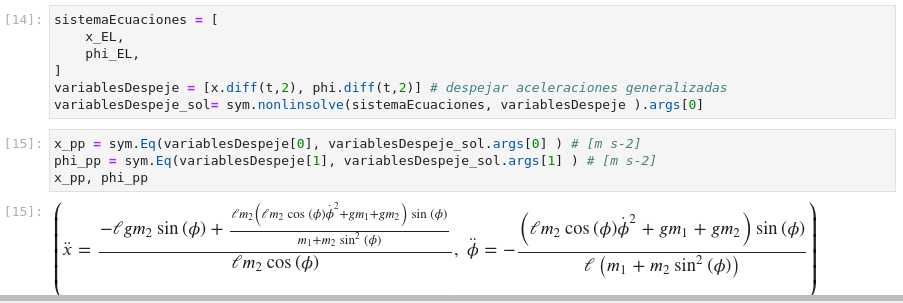
\includegraphics[width=\linewidth]{figuras/clase4Aceleraciones.png}
\caption{The resolution of systems of differential equations of certain complexity is avoided in conventional courses. In this course, it only takes a couple of lines of code with functions in the Sympy library.}
\label{fig:clase4ac}
\end{figure}



\textbf{Week 5: simulation}
Students passed a numerical analysis course to enroll in this course where such knowledge will be used.
In this lesson, the fundamentals of numerical resolution methods for differential equations are reviewed and how they would be implemented in a state vector notation suitable for efficient processing.
Immediately after the review of fundamentals, the functions of the scientific calculation library Scipy are shown in action to efficiently obtain solutions for the dynamics of a two-degrees-of-freedom system as illustrated by Figure \ref{fig:clase5sol}.

\begin{figure}[!ht]
\centering
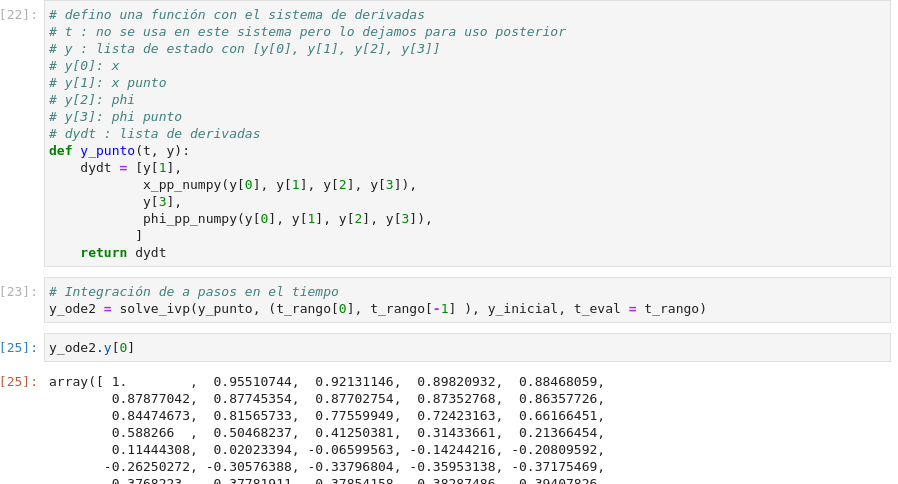
\includegraphics[width=\linewidth]{figuras/clase5Soluciones.png}
\caption{The system of equations for the dynamics of a two-degrees-of-freedom system is numerically solved with functions of the SciPy library.}
\label{fig:clase5sol}
\end{figure}

Generalized positions and velocities obtained numerically at times of interest are graphically represented, as shown by figure \ref{fig:clase5rep}, which is useful to discuss students whether the behavior of the system is consistent with what can be predicted from a qualitative analysis of this simple system.
Confirming that the symbolic and numerical calculation tools used obtain correct results gives confidence in them in view of applying this tools to more complex systems.

\begin{figure}[!ht]
	\centering
	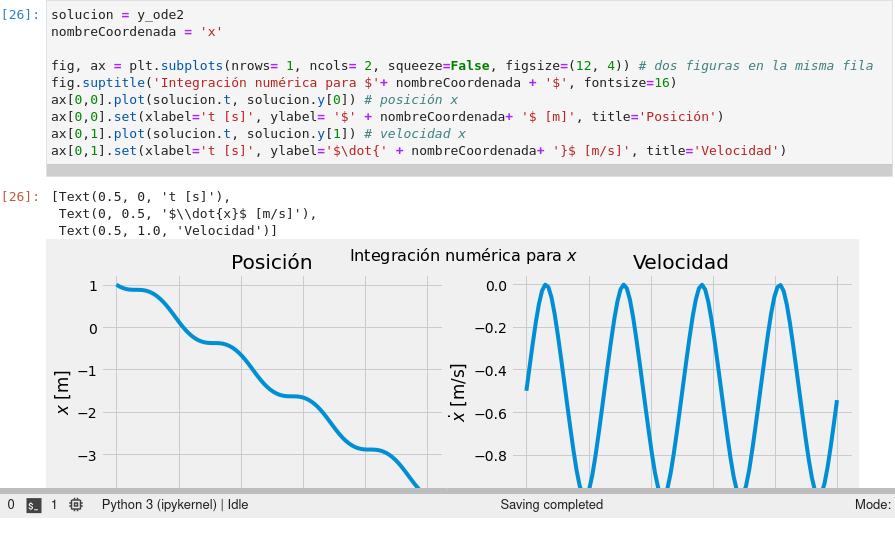
\includegraphics[width=\linewidth]{figuras/clase5Representación.png}
	\caption{
		Visualisation of results obtained by numerical calculations.
		Corroborating that what is represented corresponds to a qualitative analysis of the dynamics of the system creates confidence in the students in this tool.
	}
	\label{fig:clase5rep}
\end{figure}

\textbf{Final weeks.}
Towards the end of our course the students of our course have already developed the ability to autonomously analyse ``realistic'' systems resembling mechanical devices found in the industry.
To present them a challenge in this line, they are assigned a final project in which they must calculate the torques required for the motors of a highly simplified industrial robotic arm to perform a sequence of movements. 
Examples of the results of students' work in response to this proposal are shown in figure \ref{fig:robotarm}.

\begin{figure}[!ht]
\centering
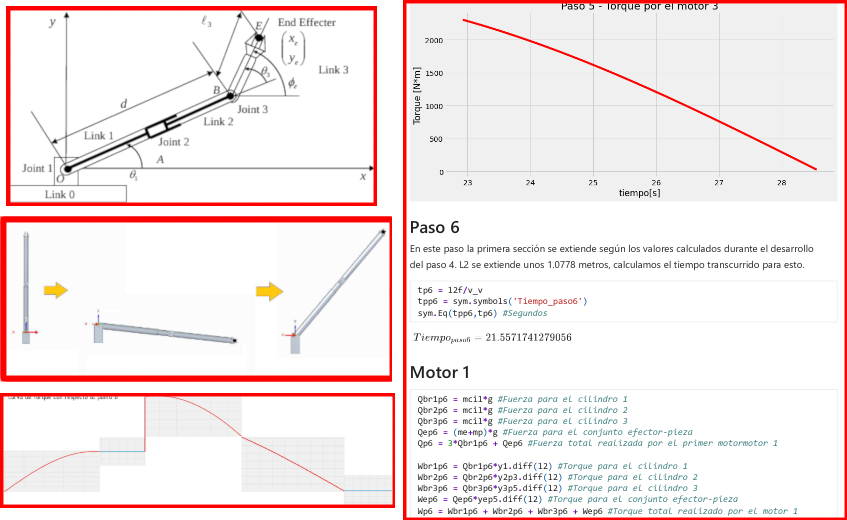
\includegraphics[width=\linewidth]{figuras/robotArm.png}
\caption{To be able to perform even a simple movement, motors of an industrial arm  must apply a sequence of torques. Students calculate them in a final assignment that reflects their mastery of analytical and computer tools taught at the course.}
\label{fig:robotarm}
\end{figure}

Students are required to present their results in an oral presentation to the teaching staff.
With this we aim to push them to improve their conmunication skills, not only by writting their work in an ordely fashion, but also to prepare a speech to defend it, a stressful situation but a must for any business-like setting.


\section{Results and objectives}

Coloque aquí los resultados alcanzados y los objetivos en curso o futuros del proyecto.

\section{Discusssion}

Desarrollo del texto.

\section{End discussion}

La exposición de teoría y la ejercitación práctica tomaron distintas ventajas de la metodología de este curso.

Clases de teoría:
\begin{itemize}
    \item La exposición en pizarrón o en una presentación en que los alumnos están concentrados en transcribir lo allí escrito se reemplazó por código que pueden reutilizar para resolver sus ejercicios.
    \item En las clases en línea cada palabra del docente durante la clase queda registrada en video  liberando al alumno de la toma de notas.
    \item El docente puede cambiar el código durante la clase para corregir un error o graficar otro aspecto de la temática.
\end{itemize}

Ejercicios de práctica:
\begin{itemize}
    \item En papel una variación sobre un ejercicio resuelto anteriormente obliga a reiterar tediosos cálculos similares. Con código basta con modificar ligeramente el mismo para atender al nuevo caso.
    \item En forma remota varios alumnos pueden trabajar concurrentemente en la resolución en un mismo ejercicio.
    \item Los alumnos pueden alertar al docente a toda hora vía el LMS de un inconveniente que enfrenten en la resolución de un ejercicio. El docente puede dedicarle tiempo y detenimiento en el momento que encuentre propicio a diferencia del acotado tiempo de consultas del que se dispone en el aula.
    \item Los docentes pueden comentar y corregir el mismo código sobre el que está trabajando el alumno inclusive en tiempo real.
\end{itemize}


\section{Conclussions}

% This is a summary of the main drivers of the course:
This course differs from conventional ones in two ways:
\begin{itemize}
    \item Code-centric% Advantages of Code-Based Learning:
    \begin{itemize}
        \item Avoids the repetitive nature of blackboard or paper based calculations. 
        \item By iteratively modifying previously tested code (initially designed for simpler mechanical systems), students expand their analytical capabilities.
        \item The complexity of the code evolves alongside the mechanical system’s intricacies introduced each class.
        \item This approach eliminates the need to \textit{start from scratch} when dealing with the extensive calculations required for analyzing complex mechanical systems using the Euler-Lagrange formalism.
        \item All systems used are currently available online on a non-cost basis, from the student point of view. Being based on free software, if any of them is later placed behind a paywall, it would be simple to run them from on the premise servers.
    \end{itemize}
    \item Flipped classroom
    \begin{itemize}
        \item Students are provided with online theory and example problems to study before weekly meetings. These asynchronous activities save classroom time for discussions and problem solving.
        \item During synchronic meetings they can rise to teachers any questions related to theory or problem-solving so they can finish their exercise sets.
        \item All exercises are turned-in for evaluation. Compliance is tracked with an online learning management system. 
    \end{itemize}
\end{itemize}
Currently, there is limited statistical data available on the impact of the course and the described methodologies.
However, feedback from students consistently indicates a high level of satisfaction, especially with the code-driven aspect of the course.
Additionally, students express interest in the final examination as it provides an opportunity to apply both their presentation skills and the knowledge acquired throughout the course.

In relation to the flipped classroom model, students acknowledge that it requires more effort, but a majority of them agree that it is a positive and beneficial implementation.
as former students assesed that the tools employed in the course were usuful to them in subsequent subjects and professional lives, the authors had consequently gained confidence on having choosed the current approach over traditional ones.


\begin{credits}
\subsubsection{\ackname} 
The authors would like to thank the coordination of the Mechanical Engineering career at DIIT-UNLaM for accompanying the development and implementation of this course. 


\subsubsection{\discintname}
The authors declare no competing interests.
\end{credits}

\printbibliography[title= Bibliography, heading=bibintoc]
%
% ---- Bibliography ----
%
% BibTeX users should specify bibliography style 'splncs04'.
% References will then be sorted and formatted in the correct style.
%
% \bibliographystyle{splncs04}
% \bibliography{mybibliography}
%
% \begin{thebibliography}{8}
% \bibitem{ref_article1}
% Author, F.: Article title. Journal \textbf{2}(5), 99--110 (2016)

% \end{thebibliography}
\end{document}
